\documentclass[12]{article}

\usepackage{graphicx}
\usepackage{algorithm}
\usepackage[noend]{algpseudocode}

\begin{document}

\title{Deep Q-Learning on Unity's Banana Environment}
\author{Christopher J. Miles}
\maketitle

%    \begin{abstract}
%    This report is done in fulfillment of the {\it Udacity Deep Reinforcement Nanodegree}. This project implements a Deep Q-Network (DQN) model and its variants such as DDQN, Dueling DQN on the Unity {\it Banana} environment. There are two observational state space encodings: ray-based perception and raw pixel information.
%    \end{abstract}




\section{Introduction}

Deep reinforcement learning (in particular, the DQN algorithm) is applied to the Unity Banana environment \cite{unity}.  The environment is a virtual 3D space where an agent is confined to a square region. The space is filled with randomly placed blue and yellow bananas. The objective is for the agent to collect as many yellow bananas as possible in the allotted time of 300 time steps. The agent receives a $+1$ reward for every yellow banana collected and a $-1$ for every blue banana collected. 

To solve this problem, variants of the Deep Q-Learning algorithm are employed \cite{Wang2016,Schaul2016,Mnih2015}. The details of each algorithms are discussed in the next section.

\section{DQN Learning Algorithms}

A `vanilla' DQN \cite{Mnih2015, Udacity2018} is implemented as follows:

\

\begin{algorithmic}[1]
\State Initialize replay memory $D$ with capacity $N$
\State Initialize action function $\hat{q}$ with random weights $w$ 
\State Initialize target action-value weights $w^{-} \leftarrow w$
 \For {the episode $e \leftarrow 1$ to $M$}
 	\State Initial input state $x_1$
	\State Prepare initial state: $S \leftarrow \phi(x_1)$
	\For {time step $t \leftarrow 1$ to $T$}
		\State Choose action $A$ from state $S$ using policy $\pi \leftarrow \epsilon-Greedy(\hat{q}(S,A,w))$
		\State Take action $A$, observe reward $R$, and next input frame $x_{t+1}$
		\State Prepare initial state: $S' \leftarrow \phi(x_{t+1})$
		\State Store experience $(S,A,R,S')$ in replay memory $D$
		\State $S \leftarrow S'$
		\State Obtain minibatch of tuples $(s_j,a_j,r_j,s_{j+1})$ from $D$ of size $K$.
		\State Set target $y_j = r_j + \gamma \max_a \hat{q}(s_{j+1}, a, w^{-})$
		\State Update $w$: $\Delta w = \alpha (y_j - \hat{q} (s_j, a_j, w))\nabla_w \hat{q}(s_j,a_j,w)$
		\State Soft update $w^{-}$: $w^{-} \leftarrow (1-\tau) w^{-} + \tau w$ 
	\EndFor
\EndFor
\end{algorithmic}

\
The function $\phi(x)$ is a feature mapping from the raw input $x$ to a vector with $37$ dimensions representing ray-based perception of objects in the agent's forward direction. The hyperparameters were set to the following: buffer size $ N = 10^{5}$, discount factor $\gamma = 0.99$, batch size $K = 64$, soft update parameter $\tau = 10^{-3}$, learning rate $\alpha =5 \times 10^{-4}$. The network used to represent $\hat{q}$ is a fully connected neural network with an input layer of $37$ nodes, a hidden layer of $64$ nodes, a second hidden layer with $64$ nodes, and the final output layer with 4 nodes (one for each action value). The activation functions were all ReLU functions with the exception of the final layer which is simply a linear combination without the addition of nonlinearity from an activation function.

The dueling DQN algorithm is identical to the algorithm above except that the neural network architecture is slightly different. The final stages of the neural network branch off to calculate the advantage of each action and state-value which is then used to determine the over all action-state values.

The double DQN algorithm is also a slight variation from the original DQN algorithm. the target $y_j = r_j + \gamma \max_a \hat{q}(s_{j+1}, a, w^{-})$ is modified to $y_j = r_j + \gamma \hat{q}(s_{j+1}, a^{*}, w^{-})$ where $a^{*} = argmax_a \hat{q}(s_{j+1},a,w)$. This change improves stability of the algorithm.

\section{Results and Plot of Rewards}
The model discussed in the previous section was implemented and resulted in the following plot shown in Figure \ref{fig:dqn}. In addition, variations of the the vanilla DQN were also implemented such as double DQN and dueling DQN. These results of these implementations are shown in figures \ref{fig:double_dqn} and \ref{fig:dueling_dqn}. From these single trial runs, there isn't a noticable differences in the length of time to achieve the solved criteria: average reward of 13 over 100 consecutive episodes. DQN solved this criteria in just over 350 episodes, Double DQN solved it in about 275 episodes, Dueling DQN solved it in about 325 episodes.


\begin{figure}
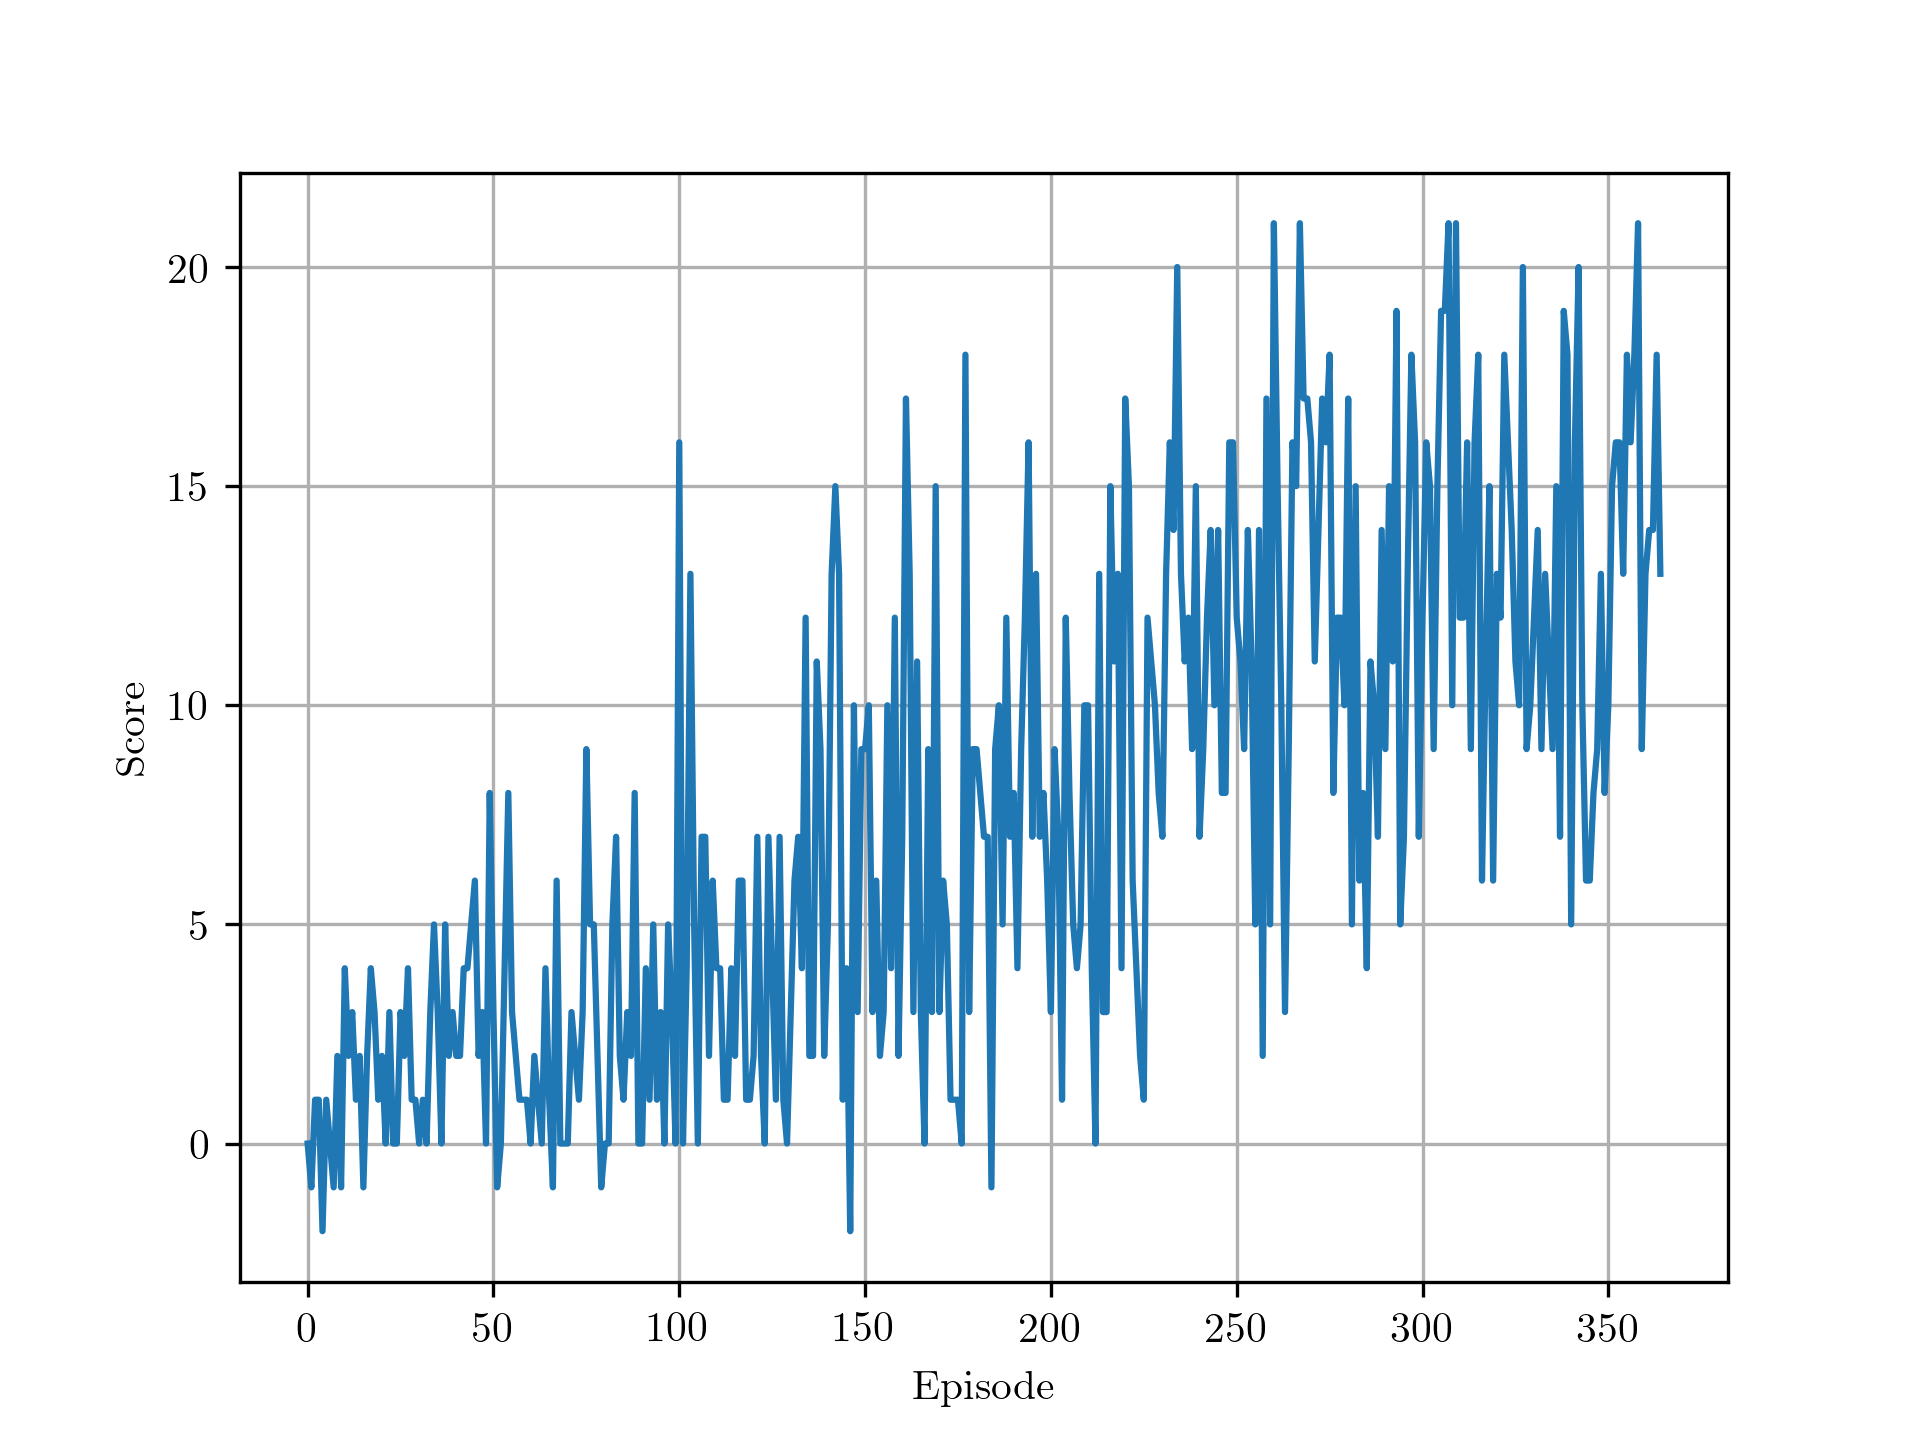
\includegraphics[width=0.9\textwidth]{images/scores_dqn}
\caption{Scores over episodes during DQN training.}
\label{fig:dqn}
\end{figure}


\begin{figure}
\includegraphics[width=0.9\textwidth]{images/scores_double_dqn}
\caption{Scores over episodes during Double DQN training.}
\label{fig:double_dqn}
\end{figure}

\begin{figure}
\includegraphics[width=0.9\textwidth]{images/scores_dueling_dqn}
\caption{Scores over episodes during Dueling DQN training.}
\label{fig:dueling_dqn}
\end{figure}

\section{Ideas for Future Work}
In future work, I would like to implement prioritized experience replay. I would also like to try learn directly from raw pixel input data rather then imposing the ray-based feature map. If I had more computational resources, I would also like to run many trials of the DQN algorithms discussed here to provide statistical averages and variances to better compare these algorithms in the statistical sense. It's hard to say much from a few single trials of a stochastic process.


\bibliographystyle{plain}
\bibliography{../library}



\end{document}